
\documentclass[letterpaper, 10 pt, conference]{ieeeconf}  

\usepackage{lmodern}
\usepackage{amsmath}
\usepackage{amsfonts}
\usepackage{graphicx}
\usepackage{cite}
\usepackage{booktabs}

\title{
\Large \bf CS405 Machine Learning\\
\huge Research Proposal\\
\vspace{0.5em}
\Large \textit{TSDR: Traffic-Sign Detection and Recognition}
}
\author{
Langchu Huang \\ 
\texttt{12213009} \\
\and
Yutong Wu \\ 
\texttt{12213012} \\
\and
Yuhang Huang \\ 
\texttt{12213015}
\and
Tianye Wu \\ 
\texttt{12211201} \\
}
\begin{document}

\maketitle

\section{Background and Significance}
\hrulefill

\subsection{Introduction}

\subsubsection{What is TSDR?}\

\textbf{Traffic Sign Detection and Recognition(TSDR)} refers to the technologies and processes used to identify and interpret various road signs and signals. It is a critical component of Intelligent Transportation Systems (ITS), Advanced Driving Assistance Systems (ADAS) and autonomous driving. TSDR enables real-time recognition and understanding of road signs, making it an essential technology for modern transportation systems.

\subsubsection{Contributions}\

TSDR plays a vital role in \textbf{Advanced Driving Assistance Systems (ADAS)}, \textbf{Autonomous Driving}, and \textbf{Intelligent Transportation Systems} by ensuring compliance with traffic rules and enhancing road safety. In ADAS, it helps vehicles provide timely warnings and navigation instructions. For autonomous driving, TSDR ensures vehicles can detect and recognize various types of signs, such as warnings, prohibitions, and instructions, contributing to a safe and efficient driving environment. Moreover, TSDR supports intelligent transportation systems by improving traffic flow and enabling the development of smart cities.

\subsubsection{Driving Technological Advancements}\

The development of TSDR promotes research in key technologies such as image recognition, deep learning, and pattern recognition. By applying these technologies to traffic sign detection, TSDR not only validates their effectiveness and adaptability but also provides valuable research experience for broader image recognition applications. Its implementation fosters innovation and accelerates progress in fields beyond transportation, making it a cornerstone for advancements in \textbf{computer vision and intelligent systems}.

\subsection{Significance}

\subsubsection{Safety}\

A report published in 2015 on Global Status Report On Road Safety by World Health Organization (WHO) showed that over 1.2 million people die across the globe annually due to road accidents \cite{WHO2015}.Traffic signs play a crucial role in ensuring road safety by providing drivers with essential information such as road conditions, speed limits, potential hazards and so on. Real-time detection and recognition of traffic signs can alert drivers to comply with traffic regulations, thereby reducing the likelihood of accidents. For example, autonomous driving systems rely on traffic sign recognition to determine whether actions such as slowing down, stopping, or yielding are required.

\subsubsection{ADAS and Autonomous Driving}\

Traffic sign detection and recognition is a key component in ADAS and autonomous driving. They must be able to recognize and interpret all traffic signs on the road to ensure the vehicle's safe operation and to make appropriate decisions in complex traffic environments. Without accurate traffic sign recognition, an autonomous system cannot reliably understand its surroundings, limiting its widespread use.

\subsubsection{Intelligent Transportation Systems}\

ITS aim to enhance traffic efficiency, reduce congestion, and minimize accidents. By using traffic sign recognition technology, traffic management systems can monitor road conditions in real time, adjust traffic signals, and provide traffic information. This not only improves traffic flow but also helps traffic authorities conduct precise traffic flow analysis and management.

\subsection{Motivations}

\begin{table*}[t!]
    \centering
    \caption{Market Size and CAGR Estimates (2024-2029)}\label{tab:market_table}
    \begin{tabular}{@{}lccc@{}}
    \toprule
    \multicolumn{4}{c}{\textbf{Market Size and CAGR Estimates (2024-2029)}} \\
    \midrule
    \textbf{Market} & \textbf{Estimated Size (2024)} & \textbf{Estimated Size (2029)} & \textbf{CAGR (2024-2029)} \\
    \midrule
    ADAS               & USD 49.65 billion  & USD 107.47 billion  & 16.70\% \\
    Autonomous driving & USD 41.10 billion  & USD 114.54 billion  & 22.75\% \\
    ITS                & USD 33.38 billion  & USD 46.36 billion   & 6.79\%  \\
    \bottomrule
    \end{tabular}
\end{table*}

\subsubsection{Technology Evolution}\

Traffic Sign Detection and Recognition (TSDR) leverages technologies such as computer vision, deep learning, and neural networks to detect and classify traffic signs. As these technologies continue to advance, TSDR systems become more accurate, efficient, and adaptable to various driving environments and conditions. At the same time, the relentless pursuit of optimization in autonomous driving algorithms also contributes to advancements in underlying technologies, fostering the development of the entire technical ecosystem.

With the increase in computational power and the efficiency of algorithms, TSDR can now operate in real-time. This is critical for autonomous vehicles and Advanced Driver-Assistance Systems (ADAS), which rely on the rapid and accurate detection of traffic signs. 

\subsubsection{Commercial Value}\

TSDR, as an important part in ADAS, autonomous driving, and ITS, has immense commercial value. Several studies from Mordor Intelligence Table~\ref{tab:market_table} shows that, The Advanced Driver Assistance Systems Market size is estimated at USD 49.65 billion in 2024, and is expected to reach USD 107.47 billion by 2029, growing at a CAGR of 16.70\% during the forecast period (2024-2029) \cite{Mordor2024ADAS}. The Autonomous Car Market size is estimated at USD 41.10 billion in 2024, and is expected to reach USD 114.54 billion by 2029, growing at a CAGR of 22.75\% during the forecast period (2024-2029) \cite{Mordor2023Autonomous}. The Smart Transportation Market size is estimated at USD 33.38 billion in 2024, and is expected to reach USD 46.36 billion by 2029, growing at a CAGR of 6.79\% during the forecast period (2024-2029) \cite{Mordor2024SmartTransportation}.

\
\section{Analysis of Current Research Status}
\hrulefill

\subsection{Datasets and Benchmarks}

\subsubsection{Foreign}\

\textbf{Road-sign-detection Dataset} \cite{make_ml}:

Contains 877 images across 4 classes for road sign detection. Bounding box annotations are provided in the PASCAL VOC format.

\textbf{GTSDB (German Traffic Sign Detection Benchmark) Dataset} \cite{Houben-IJCNN-2013}:

Released by Karlsruhe Institute of Technology (KIT), Germany. A large-scale dataset with 5183 images of 43 distinct traffic sign types from real-world traffic scenarios in Germany. Split into 4080 training images and 1103 testing images. Each image includes bounding box annotations and the corresponding sign type. The dataset also provides evaluation metrics for comparing model performance.

\textbf{BTSD (Belgium Traffic Sign Dataset) Dataset} \cite{timothefe2013traffic}:

Released and hosted by VISICS, ESAT, KU Leuven. Contains 900 images of traffic signs, categorized into 4 main classes: Prohibited, Hazard, Mandatory, and Other, with 42 sub-classes.

\textbf{LISA (LISA Traffic Sign Dataset)} \cite{mogelmose2012lisa}:

Consists of images and video frames for traffic sign detection, with annotations for 47 types of traffic signs. The dataset includes 6610 frames with 7855 annotations. Image sizes vary from 640x480 to 1024x522 pixels. Annotations include sign type, position, size, occlusion status, and whether the sign is on a secondary road. The complete dataset includes video frames along with images.

\subsubsection{Chinese}\

\textbf{TT100K Dataset} \cite{Zhe_2016_CVPR}:

A large-scale traffic sign dataset containing 100,000 images. The dataset includes more than 200 classes of traffic signs, with a diverse range of traffic signs from multiple countries. Annotations are in bounding box format, providing detailed information on each sign's location and class. The dataset is designed for both traffic sign detection and recognition tasks.

\textbf{CCTSDB (Chinese City Traffic Sign Database) Dataset} \cite{zhang2024robust}

Contains more than 10,000 images with over 60 categories of Chinese traffic signs. Includes real-world traffic sign images from urban environments in China. Annotated with bounding boxes and detailed labels for each traffic sign. The dataset is intended for traffic sign recognition and detection, focusing on challenges specific to urban Chinese environments, such as diverse traffic signs and variable lighting conditions.

\subsection{Models Architecture and Principle}

\subsubsection{Traditional Computer Vision Method}\

\textbf{Color and Shape Analysis}

Based on the traditional computer vision method, traffic sign detection can be achieved by the color and shape analysis (Figure~\ref{fig:color_shape} \cite{swathi2017automatic}). Color segmentation process eliminates the unnecessary objects and hence it reduces the search area of the image or video frame. The color distance is defined, similar to the Euclidean distance between two points and it is calculated by taking the difference between the two colors, and as the color distance decreases the similarity increases.each pixel in the RGB space is compared with the threshold values defined for each component. Only the component value larger than the threshold is converted to 255 otherwise it is set to 0. Hence, the picture is eliminated, through thresholding in color spaces like RGB, HSV, or this time, HSV can achieve a maximum detective speed of 95\% .

\begin{figure}[!t]
    \centering
    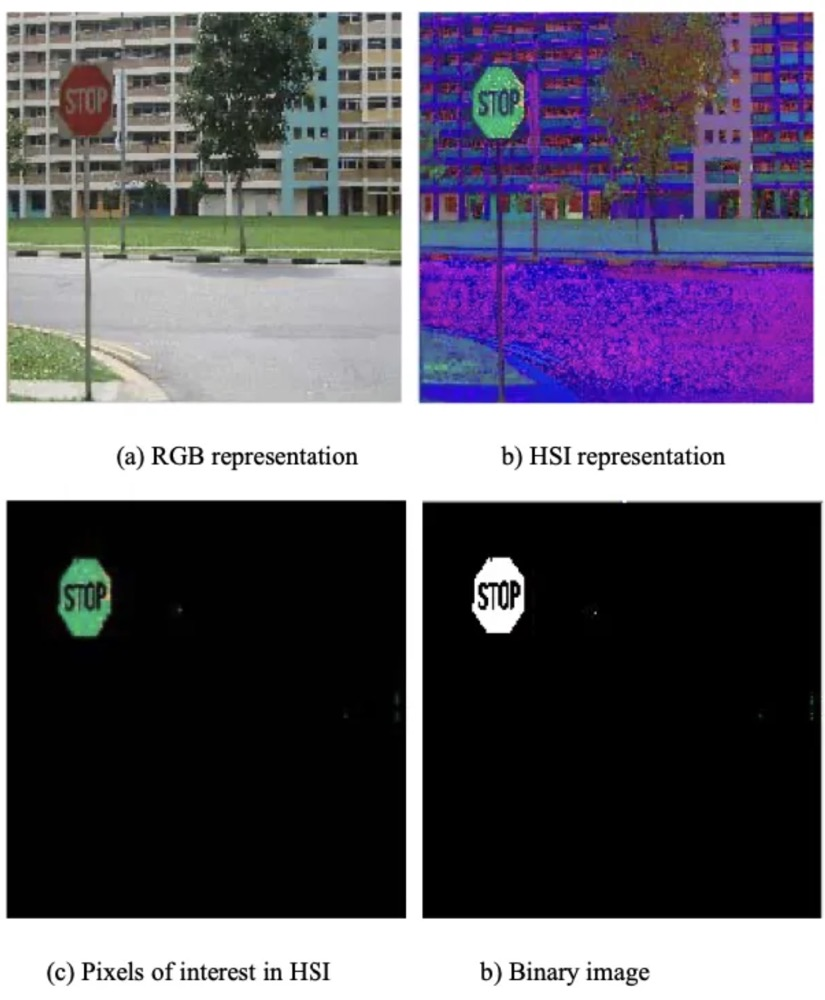
\includegraphics[width=0.9\linewidth]{figures/color_shape.jpg} 
    \caption{Color and Shape Analysis.}
    \label{fig:color_shape}
\end{figure}

As for the shape analysis, it can eliminate the issue in color based detection is the ambient illumination variation since generally traffic signs are triangle, rectangle, octagon and circular using Hough transform, detection rates of 97.2\% and 94.3\% (Figure~\ref{fig:three_kind}) are achieved for the speed limit and warning signs respectively \cite{Swathi2017}.

\begin{figure}[!t]
    \centering
    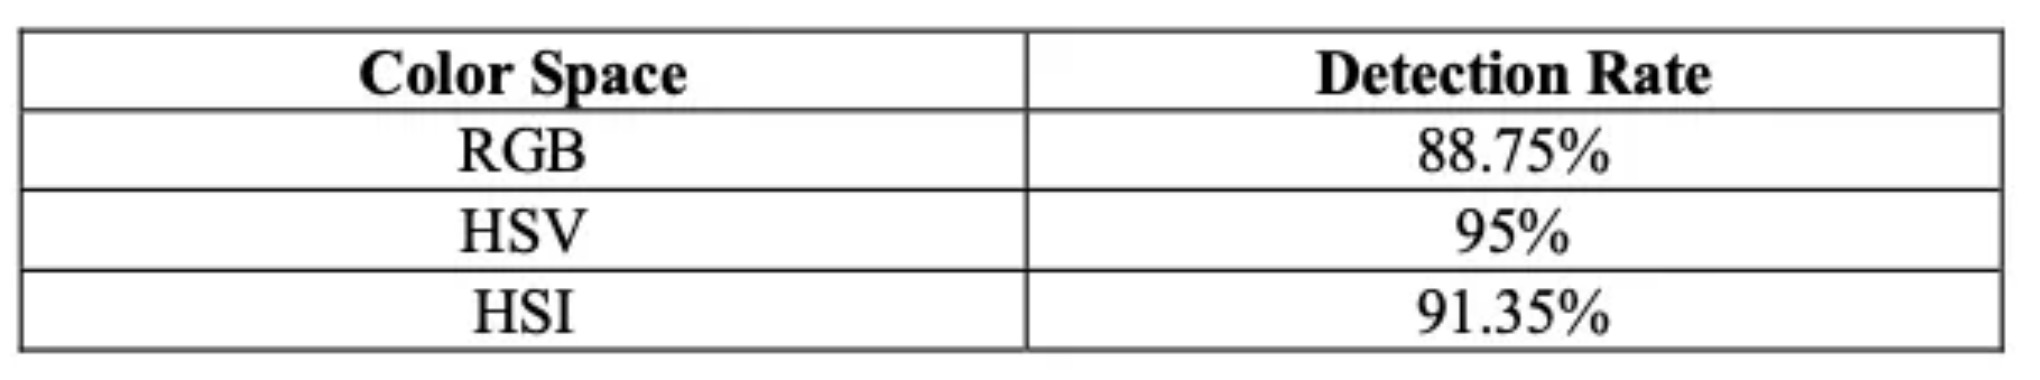
\includegraphics[width=0.9\linewidth]{figures/color_rate.jpg} 
    \caption{Three Kinds of Color Detection.}
    \label{fig:three_kind}
\end{figure}

There are also some other color and shape analysis(Figure~\ref{fig:color_based_method} Figure~\ref{fig:shape_based_method} \cite{liu2019machine}):

\begin{figure*}[!t]
    \centering
    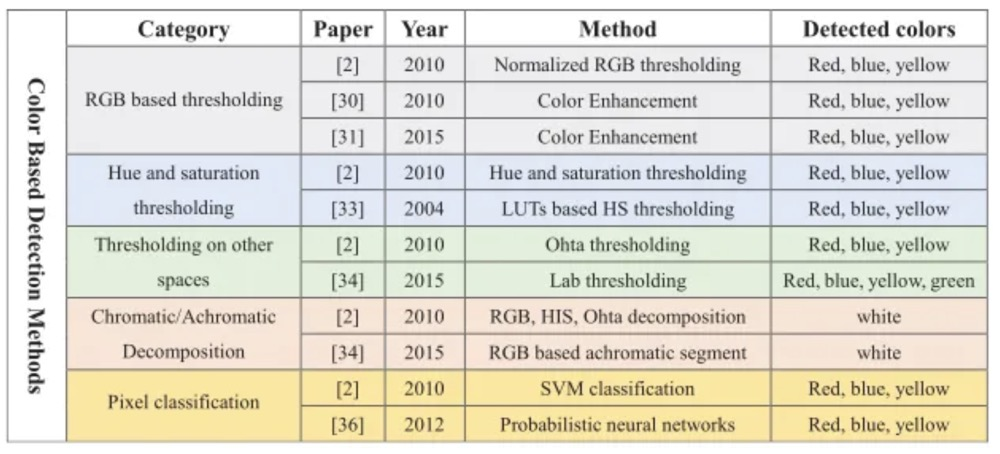
\includegraphics[width=0.9\textwidth]{figures/color_based_method.jpg} 
    \caption{Color Based Detection Method.}
    \label{fig:color_based_method}
\end{figure*}

\begin{figure*}[!t]
    \centering
    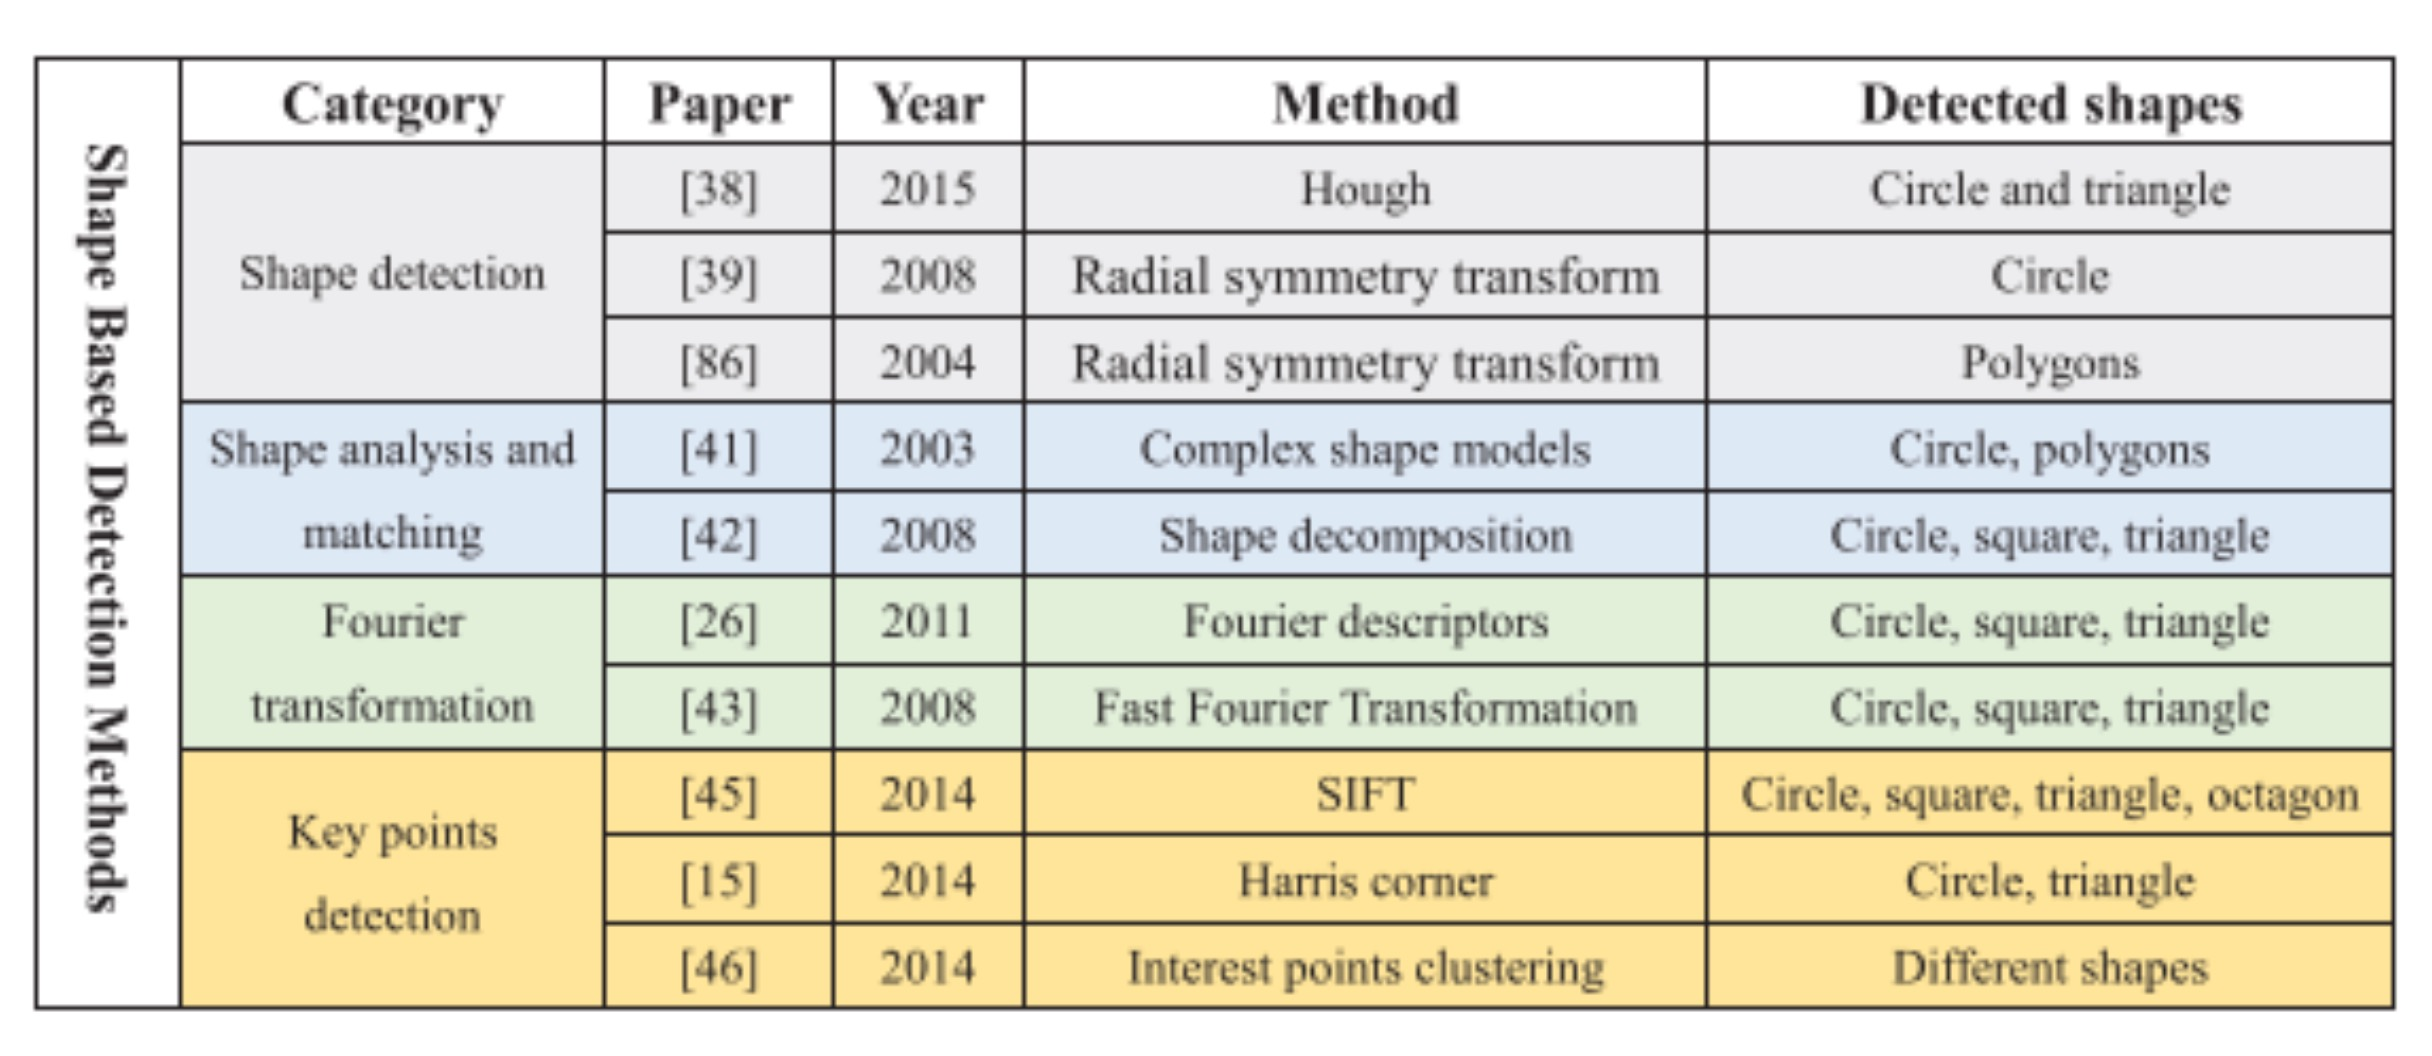
\includegraphics[width=0.9\textwidth]{figures/shape_based_method.jpg} 
    \caption{Shape Based Detection Method.}
    \label{fig:shape_based_method}
\end{figure*}

When it comes to the recognition part, it can be done either by using feature matching algorithms or by using machine learning algorithms.Artificial Neural Networks are built with the inspiration of biological neurons. Intelligent behaviour of human beings is attributed to the biological neural network. This kind of system is implemented artificially by using Artificial Neural Network (ANN). The authors \cite{Supreeth2016} in used the auto-associative neural network to recognize the traffic signs in video frames and achieved a recognition rate of 100\% and 94.7\% in both daylight and shadow environment

\textbf{Feature-Based Methods}

The SVM and Histograms of Oriented Gradients (HOG) (Figure~\ref{fig:hog_descriptor}) \cite{Swathi2017} based detection structure was first proposed to detect pedestrians and has been commonly used in different detection problems in the past decade. This structure utilizes HOG-like features to express the objects and treats the object detection problem as an SVM classification problem, in which each candidate is classified into objects or backgrounds.

\begin{figure}[!t]
    \centering
    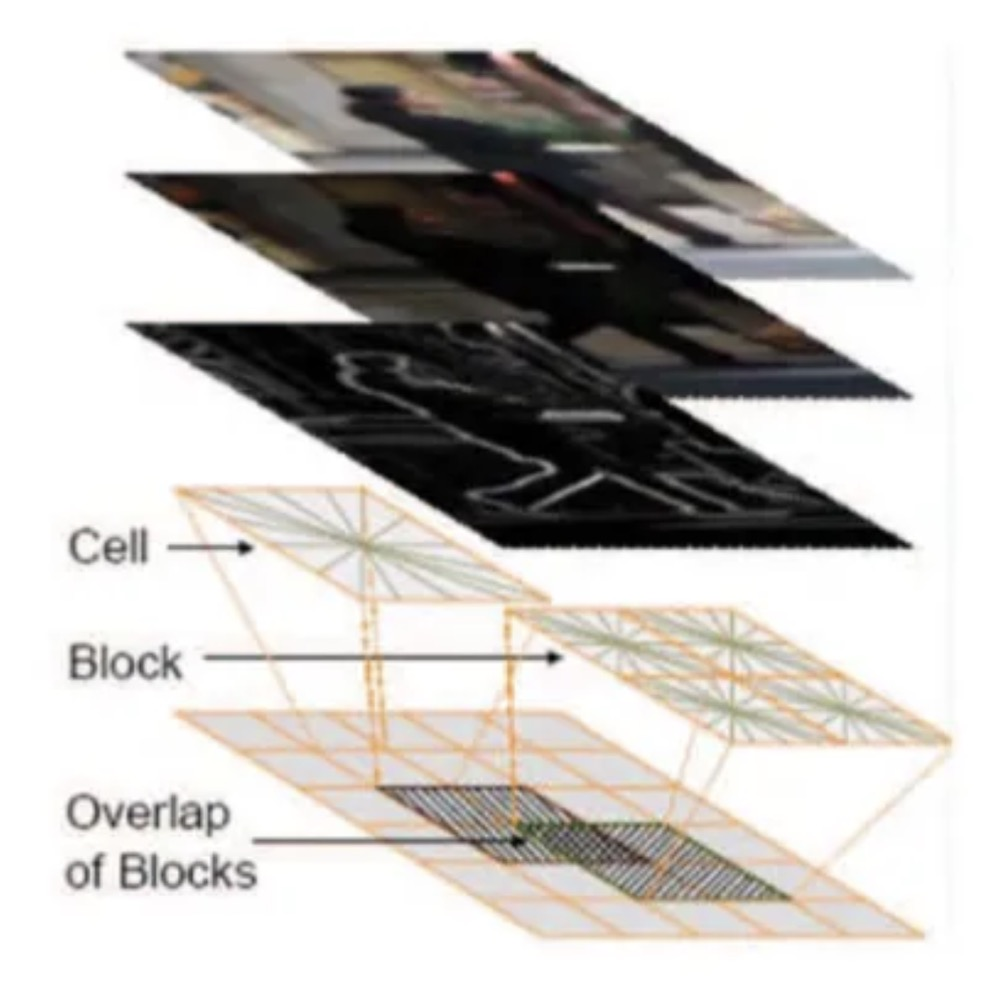
\includegraphics[width=0.9\linewidth]{figures/hog_descriptor.jpg} 
    \caption{HOG descriptor.}
    \label{fig:hog_descriptor}
\end{figure}

The SVM based detection structure has been successfully applied in TSD problems.The introduction of HOG-like features is the key of the success of SVM based detection methods. The HOG feature \cite{Dalal2005} is the most popular feature used in different detection problems. Using classical HOG features, the HOG+SVM based detection methods \cite{Salti2015}, \cite{Zaklouta2014} can achieve high detection results. Using different HOG features can generate more vectors for SVM classification. If different HOG features can express objects well, the performance may be improved. An exhaustive scanning process is used in the SVM-based detection process, which is a time-consuming process for scanning a high-resolution image. Hence, most SVM based detection methods have a ROI extraction process, which can largely reduce the scanning regions saving detection time. In \cite{Zaklouta2014}, color enhancement and MSERs based method was utilized to extract ROIs and applied SVM+HOG detector to classify the ROIs as objects or backgrounds. Many ROI extraction methods for SVM detectors have been described in the color or shape based detection parts in this review. Furthermore, methods based on SVM and HOG also play an important role in the classification of shapes, normal signs and occluded signs \cite{Hou2017}.


\textbf{Ensemble learning}

Viola and Jones' AdaBoost and cascade based detection structure (VJ) \cite{Salti2015} has been proved very efficient in some object detection problems, such as face detection, car detection, license plate detection, etc. This structure has also been successfully applied in different TSD applications.Combined with some types of rectangular features, an AdaBoost based learning method and a cascade structure, the VJ structure can select features with the AdaBoost method for object expression and then detect objects in a cascade process.

\begin{figure}[!t]
    \centering
    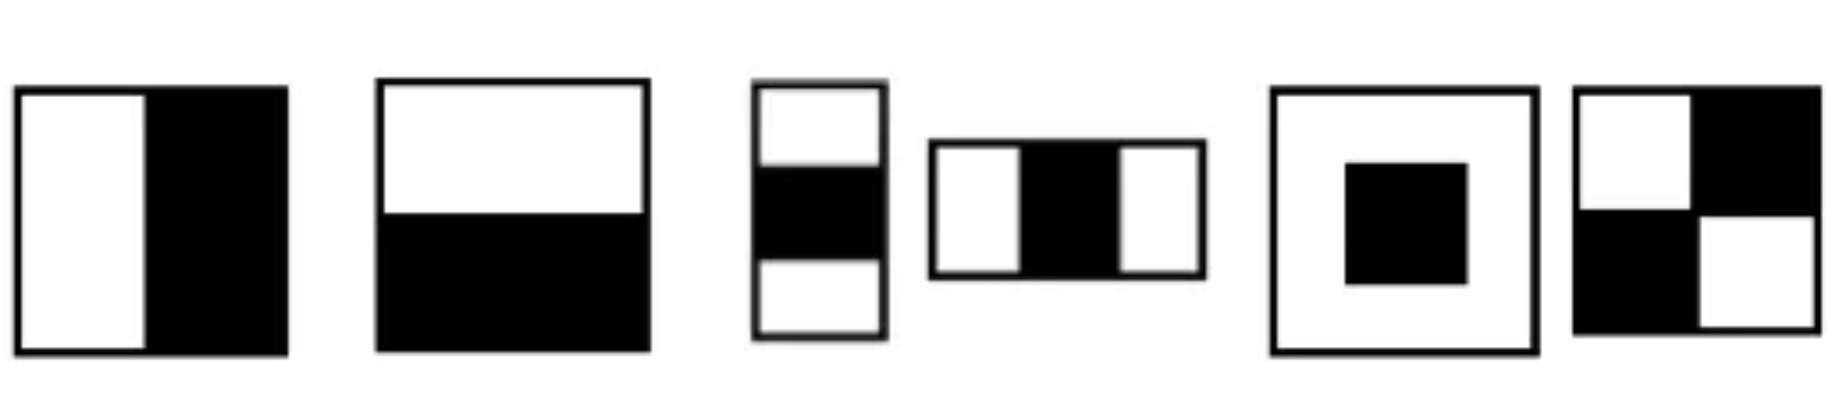
\includegraphics[width=0.9\linewidth]{figures/haar_feather.jpg} 
    \caption{Haar Like Feather.}
    \label{fig:haar_like_feather}
\end{figure}

The selection of features is crucial for AdaBoost based TSD detectors. The Haar-like feature \cite{Dalal2005} is the most popular feature used in different detection problems. The Haar-like feature can express the gray level difference of traffic signs. \cite{Salti2015} Considering that Haar-like features have connected dipoles, Baróet al.proposed the dissociated dipoles feature, which is a more general rectangular feature. Using uncon- nected two dipoles, the dissociated dipoles feature can pro- duce more features to express traffic signs. Multi-Block Local

\begin{figure}[!t]
    \centering
    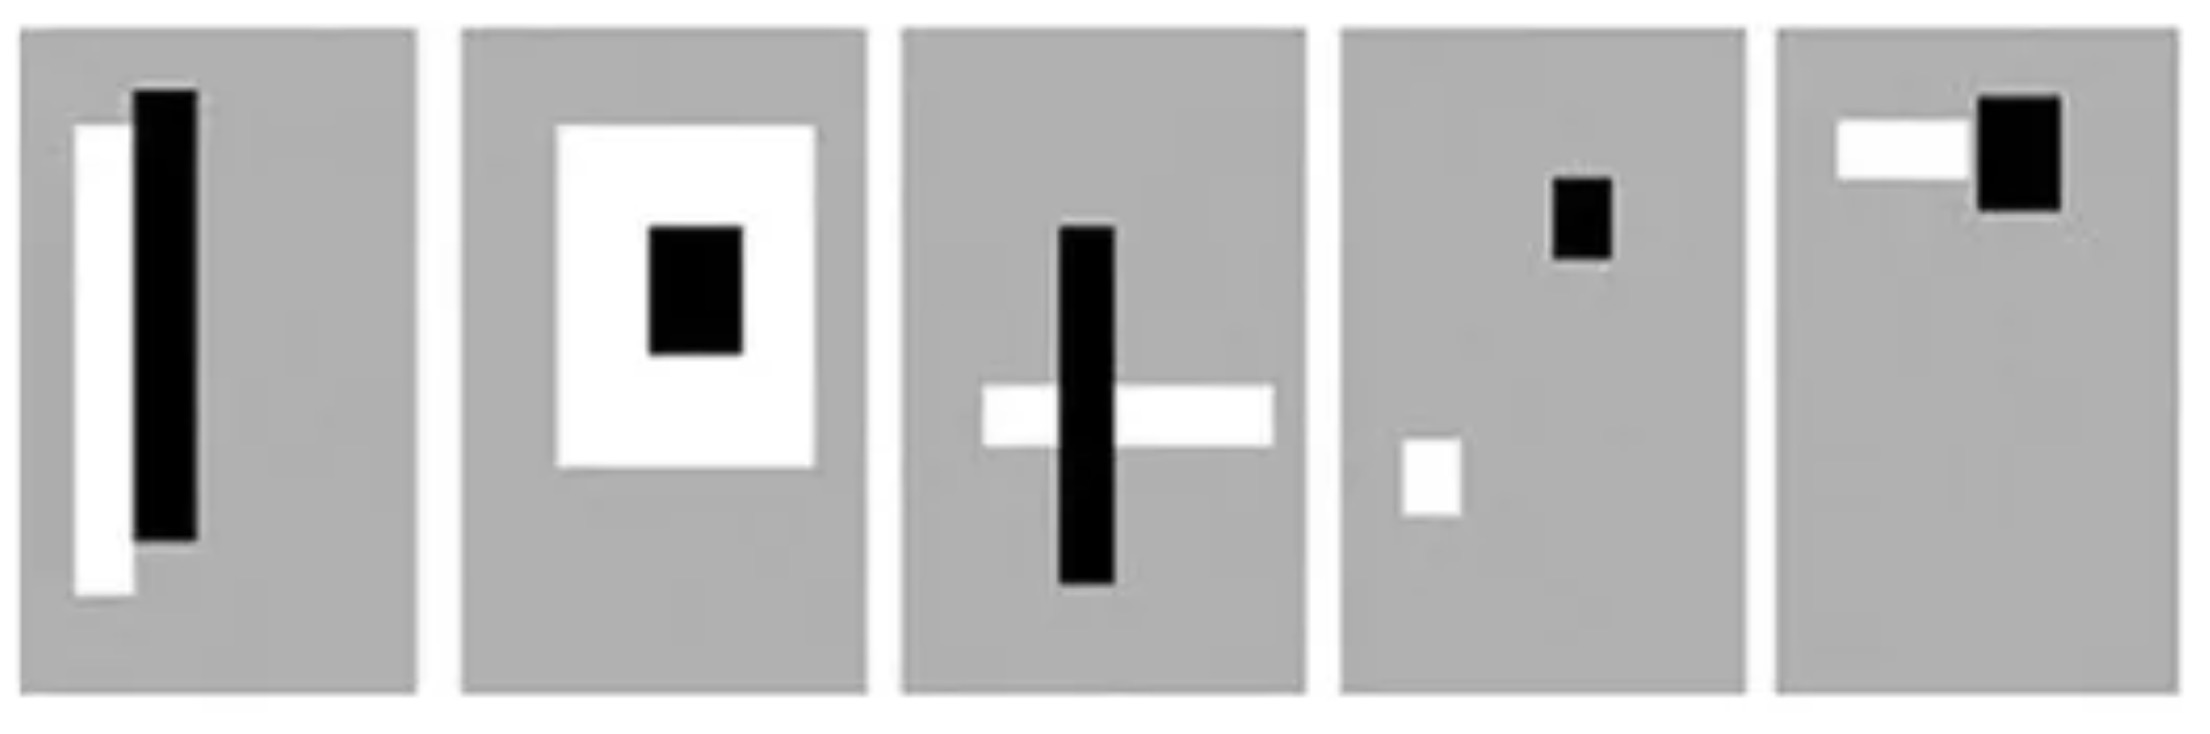
\includegraphics[width=0.9\linewidth]{figures/dissociated_dipoles.jpg} 
    \caption{Dissociated Dipoles.}
    \label{fig:dissociated_dipoles}
\end{figure}

Binary Pattern (MB-LBP) feature \cite{Zaklouta2014} is another popular used rectangular features. Liuet al. \cite{Hou2017} designed multi-block normalization LBP (MN-LBP) features to express different types of features. The designed MN-LBP feature can be trained to find the common features of different types of traffic signs.

The structures of the Haar-like features, dissociated dipoles, MN-LBP, ICF and ACF are shown above figures

The common AdaBoost based training methods include Real AdaBoost, Gentle AdaBoost, Discrete AdaBoost and other derived Boosting methods. These AdaBoost training methods can select powerful features as weak classifiers, which can form a strong classifier for object detection.Though AdaBoost based detection is very fast, scanning a high-resolution image is still time-consuming.

Finally, here is a comparison of the above 4 kind of method(Figure~\ref{fig:review} \cite{Liu2019}):

\begin{figure*}[!t]
    \centering
    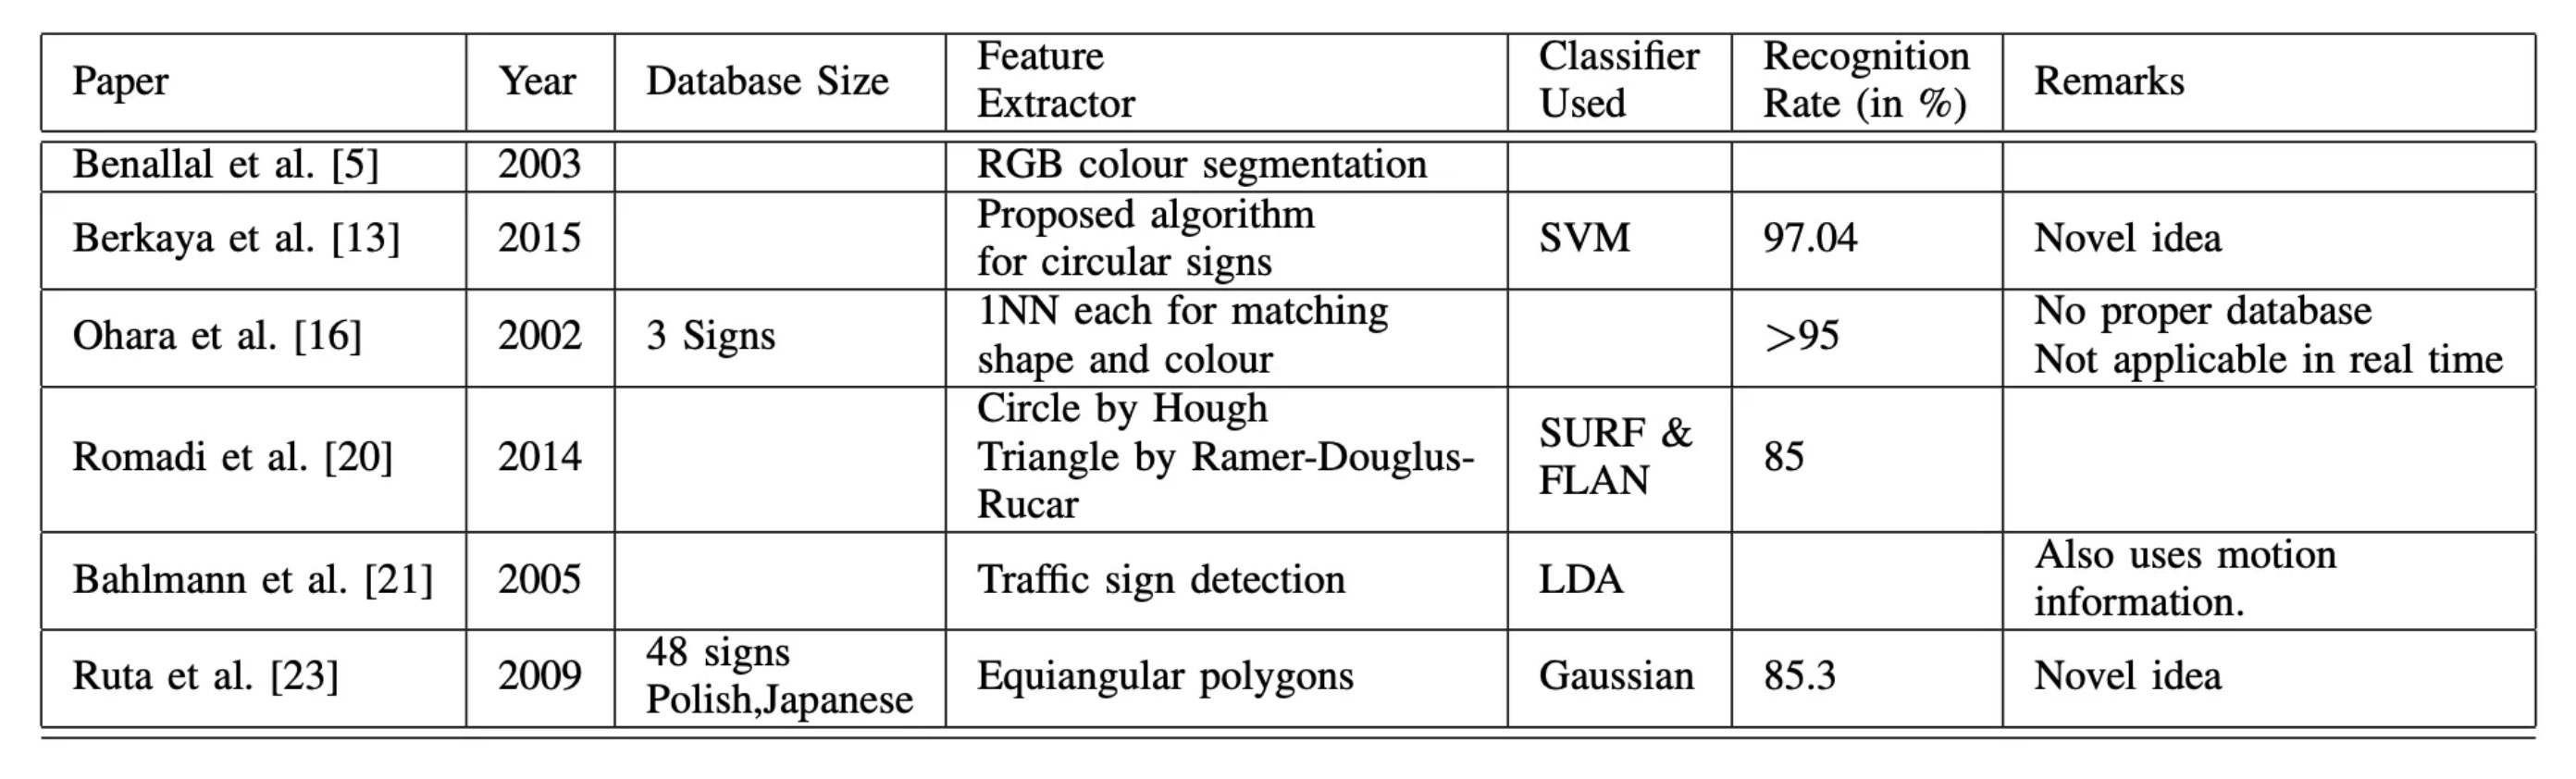
\includegraphics[width=0.9\textwidth]{figures/review.jpg} 
    \caption{Review of Techniques that Use Shape and Color for Detection.}
    \label{fig:review}
\end{figure*}

\subsubsection{The Novel Deep Learning-base Method}\

The Convolutional Neural Network (CNN) based detection methods learn features through convolutional networks. In recent years, with the development of deep learning, many different deep neural network structures have appeared and made breakthroughs in different detection areas. The use of CNN for the TSD problem started in \cite{Wu2013} and \cite{Qian2015}. These works use a CNN classifier to classify objects from backgrounds and need ROIs extraction methods to get candidates. Nowadays, there are some networks that have fast performance, such as You Only Look Once (YOLO) net. Zhang et al. \cite{Zhang2017} utilized YOLOv2 to design their real-time traffic sign detection method. Liu et al. \cite{Liu2024} used a YOLO CNN to classify traffic signs and MSRCR image augmentation during pre-processing. In the improvement phase, they used YOLOv5 to automate traffic sign categorization and improved training methods and network architecture. It achieved a 99.8\% accuracy rate on the GTSRB dataset and 98.4\% precision on the CCTSDB. Wang et al. \cite{Wang2024} separated the proposed deep ensemble learning algorithm into two methods. First, after the traffic scene process, the algorithm detects the traffic sign as two categories with the YOLOv5s network. Then, it processes the traffic sign to recognize the traffic sign into seven classes using the MobileNet network. The result of the proposed algorithm showed high performance, with 95.83\% accuracy, 87.34\% true prediction, and 191.3 milliseconds (ms) of inference time. Sharma and Kumar’s study \cite{Sharma2024} provides YOLOv8 for traffic signal recognition in the advanced version that operates in a real-time environment for road safety improvement. Intensively and widely tested and trained using a complex set of data, the YOLOv8 model gained a notable boost over its predecessors in key performance metrics such as precision, recall, and F1-score. The system performed extremely well, with the F1 score being 90.18\%, recall of 89.5\%, natural and language translation error rates of 5\%, and precision of 91\%, with only 2\% errors.

\subsubsection{Comparasion}\

Here is a comparison of the performance  of the above method, which expressed by different dataset. (Figure~\ref{fig:comparasion} \cite{Liu2019}):

\begin{figure*}[!t]
    \centering
    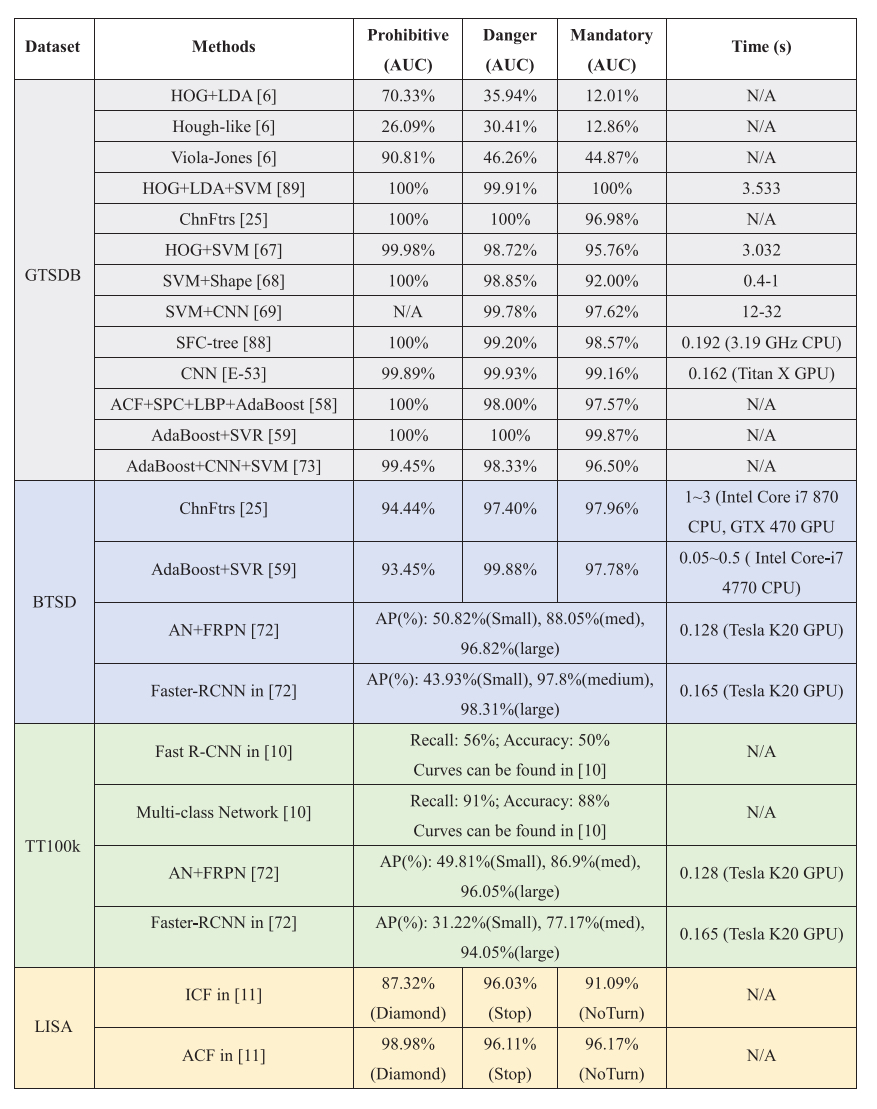
\includegraphics[width=0.9\textwidth]{figures/comparasion.jpg} 
    \caption{Review of Techniques that Use Shape and Color for Detection.}
    \label{fig:comparasion}
\end{figure*}

\subsection{Reproduction of Current Paper}

\subsubsection{Reproduction and Analysis of \cite{arcos2018deep}}\

We have selected this paper for reproduction because it introduces a versatile plug-and-play module in the domain of recognition tasks. The underlying model is a CNN, a well-known architecture for image recognition, and our target model, YOLO, is a specialized form of CNN. Our intention is to integrate this module into our final model.

One of the compelling reasons for choosing this paper is its significant experiments on optimizers, particularly the relationship between training speed and the performance of the final model. These insights could potentially help us reduce training time and achieve superior performance.

The core of the paper revolves around STPs (\textbf{Spatial Transformer Networks}):
\begin{itemize}
    \item A modular component designed to dynamically manage geometric transformations.
    \item Consists of three key components: Localization Network, Grid Generator, and Sampler.
    \item Enhances robustness by adjusting inputs to facilitate better feature extraction.
    \item In summary, this module is well-suited for any CNN to mitigate the effects of dynamically distorted figures. STNs are not only beneficial for traffic sign recognition but also applicable to other tasks demanding geometric invariance.
\end{itemize}

Based on our optimizer experiment outcomes, we concur with the paper's findings:

\begin{itemize}
    \item SGD necessitates meticulous learning rate tuning and shows slower convergence.
    \item Adam demonstrated the quickest convergence and delivered the best overall performance.
    \item RMSprop outperformed SGD in certain situations but was marginally less effective than Adam.
    \item In conclusion, Adam's adaptability makes it an optimal choice for irregular datasets, while SGD remains a strong contender for large-scale datasets with proper tuning.
\end{itemize}


\subsubsection{Reproduction and Analysis of \cite{zhang2017real}}\

We have selected this paper for reproduction because it introduces significant improvements to the YOLOv2 algorithm, specifically tailored for real-time Chinese traffic sign detection. YOLOv2 is a powerful and widely used architecture in object detection, and its modifications in this paper offer practical advancements in handling the diverse and challenging conditions of traffic sign detection. Our goal is to integrate these optimizations into our traffic sign recognition YOLOv5 model to enhance detection performance and real-time capabilities.

A major reason for choosing this paper is its focus on optimizing YOLOv2 for real-time applications, particularly for Chinese traffic signs, which involve unique challenges such as varying sign sizes, lighting conditions, and sign types. The proposed modifications allow the model to maintain high detection accuracy while operating efficiently in real-time scenarios, which is crucial for autonomous driving and intelligent transportation systems.

The core contributions of the paper are the following key improvements to YOLOv2:
\begin{itemize}
    \item \textbf{Network Architecture Modification:}
    \begin{itemize}
        \item The architecture of YOLOv2 is adapted to improve feature extraction, especially for small or obscured traffic signs. This modification boosts the model's ability to detect hard-to-spot signs that might otherwise be missed.
    \end{itemize}
    \item \textbf{Post-Processing Optimization:}
    \begin{itemize}
        \item Post-processing techniques are improved to better handle bounding box predictions, reducing false positives and enhancing the precision of detected traffic signs.
    \end{itemize}
    \item \textbf{Custom Traffic Sign Dataset:}
    \begin{itemize}
        \item The paper uses a customized dataset containing a diverse set of Chinese traffic signs, which helps the model generalize better to the variety of signs encountered in the real world.
    \end{itemize}
\end{itemize}
Based on our reproduction experiments, we observe similar results to the paper's findings:
\begin{itemize}
    \item \textbf{Real-Time Performance:}
    \begin{itemize}
        \item The model retains YOLOv2's real-time performance while achieving a noticeable improvement in detection accuracy, especially for small and distant traffic signs.
    \end{itemize}
    \item \textbf{Robustness to Different Conditions:}
    \begin{itemize}
        \item The preprocessing and multi-scale detection enhancements enable the model to perform well in diverse environments, including varying lighting and weather conditions, which is critical for real-time applications.
    \end{itemize}
\end{itemize}


\textbf{Feature-Based Methods}
\textbf{Feature-Based Methods}
\textbf{Feature-Based Methods}
\textbf{Feature-Based Methods}

\

\
\section{Completed Work}
\hrulefill

\subsection{Model selection}

For the Traffic Sign Detection and Recognition (TSDR) problem, we have selected YOLOv5 as the base model. The choice of YOLOv5 is based on several key factors:

\subsubsection{Deep Learning Revolution in TSDR}\
Traditionally, traffic sign detection and recognition were approached using traditional machine learning techniques such as support vector machines (SVM), k-nearest neighbors (KNN), and feature-based methods like Histogram of Oriented Gradients (HOG). While these methods provided decent results in controlled settings, they struggled with real-world complexities such as variations in lighting, occlusions, and different sign sizes. In recent years, deep learning techniques, especially Convolutional Neural Networks (CNNs), have become the go-to approach for image recognition tasks, including traffic sign detection. CNNs, with their ability to automatically learn hierarchical features from raw images, have significantly outperformed traditional methods.

\subsubsection{Advantages of YOLO}\
YOLO is a state-of-the-art deep learning model known for its speed and accuracy in object detection tasks. Unlike other object detection algorithms, YOLO frames the detection problem as a single regression problem, which enables it to process images in real-time. This is especially important for TSDR, where the system needs to identify and locate traffic signs accurately and quickly in dynamic environments, such as moving vehicles or changing road conditions.

\subsubsection{Why YOLOv5?}\
\textbf{Efficiency and Speed}
YOLOv5 is a further improvement on the original YOLO architecture and offers a good balance between speed and accuracy. It is lightweight, fast, and capable of real-time detection, which is crucial for deployment in autonomous driving systems or traffic monitoring systems.

\textbf{State-of-the-Art Performance}
YOLOv5 has been proven to achieve state-of-the-art performance on object detection tasks, including those in complex, real-world scenarios. This makes it particularly suitable for the TSDR task, where traffic signs need to be detected under diverse conditions such as varying sign sizes, angles, and environmental factors (e.g., night-time, rainy weather).

\textbf{Flexibility for Deployment}
YOLOv5 is highly flexible and can be easily integrated into a variety of deployment environments, whether it be in a real-time application in a vehicle or on a cloud-based monitoring system. This ease of deployment ensures that our model can be tested and used in real-world traffic scenarios without major adjustments to the underlying architecture.

\subsubsection{Support for Transfer Learning}\

YOLOv5 also supports transfer learning, allowing us to fine-tune the model with traffic sign-specific datasets. This is essential for improving the model's accuracy when dealing with the specific types of signs found in our targeted region (e.g., Chinese traffic signs) or in diverse traffic environments.
    
In conclusion, YOLOv5 was chosen as the base model for TSDR due to its impressive balance of speed, accuracy, and flexibility, making it well-suited for real-time, large-scale deployment in traffic sign recognition systems.

\subsection{Model principle}

\subsubsection{YOLOv5 Architecture}\

\begin{figure}[!t]
    \centering
    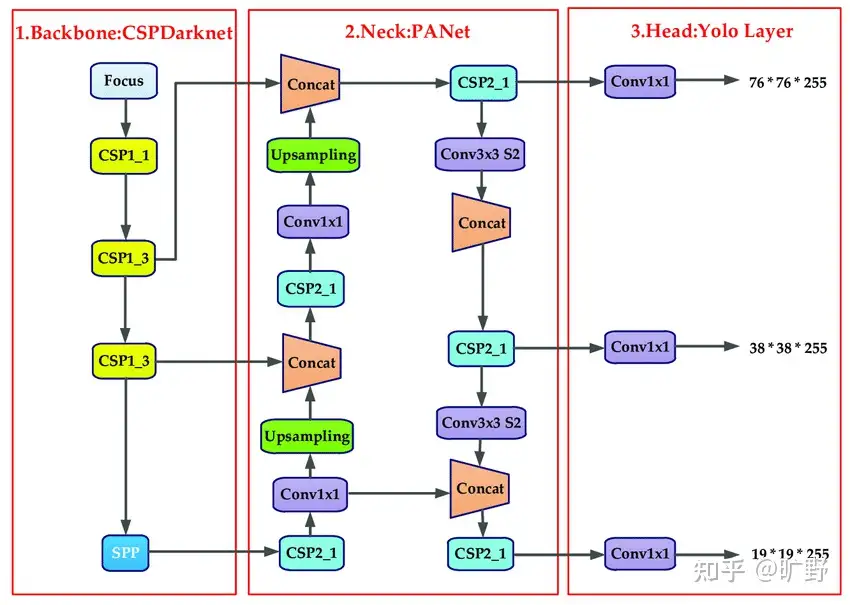
\includegraphics[width=0.9\linewidth]{figures/yolov5.png} 
    \caption{YOLOv5 architecture.}
    \label{fig:yolov5}
\end{figure}

YOLOv5 leverages a fully convolutional neural network (CNN) to process the image and make these predictions. The architecture can be broken down into several key components as shown in Figure~\ref{fig:yolov5}:

\textbf{Backbone:}
The backbone network extracts features from the input image. YOLOv5 uses CSPDarknet53 as kits backbone, a variant of Darknet53 that introduces Cross-Stage Partial Networks (CSP) to enhance feature propagation and reduce the computational load.
\textbf{Neck:}
The neck in YOLOv5 uses the PANet (Path Aggregation Network) to combine feature maps from different layers, allowing the model to leverage both low-level and high-level features. This helps the model make more accurate predictions, especially for small or distant objects.
\textbf{Head:}
The head of the network is responsible for making the final predictions (bounding box, class probability, and object confidence) from the features extracted by the backbone and aggregated by the neck.


The output from the model consists of a set of predicted bounding boxes with associated class labels and confidence scores, allowing the system to perform object detection.

\subsubsection{Key Variants of YOLOv5}\

\begin{figure}[!t]
    \centering
    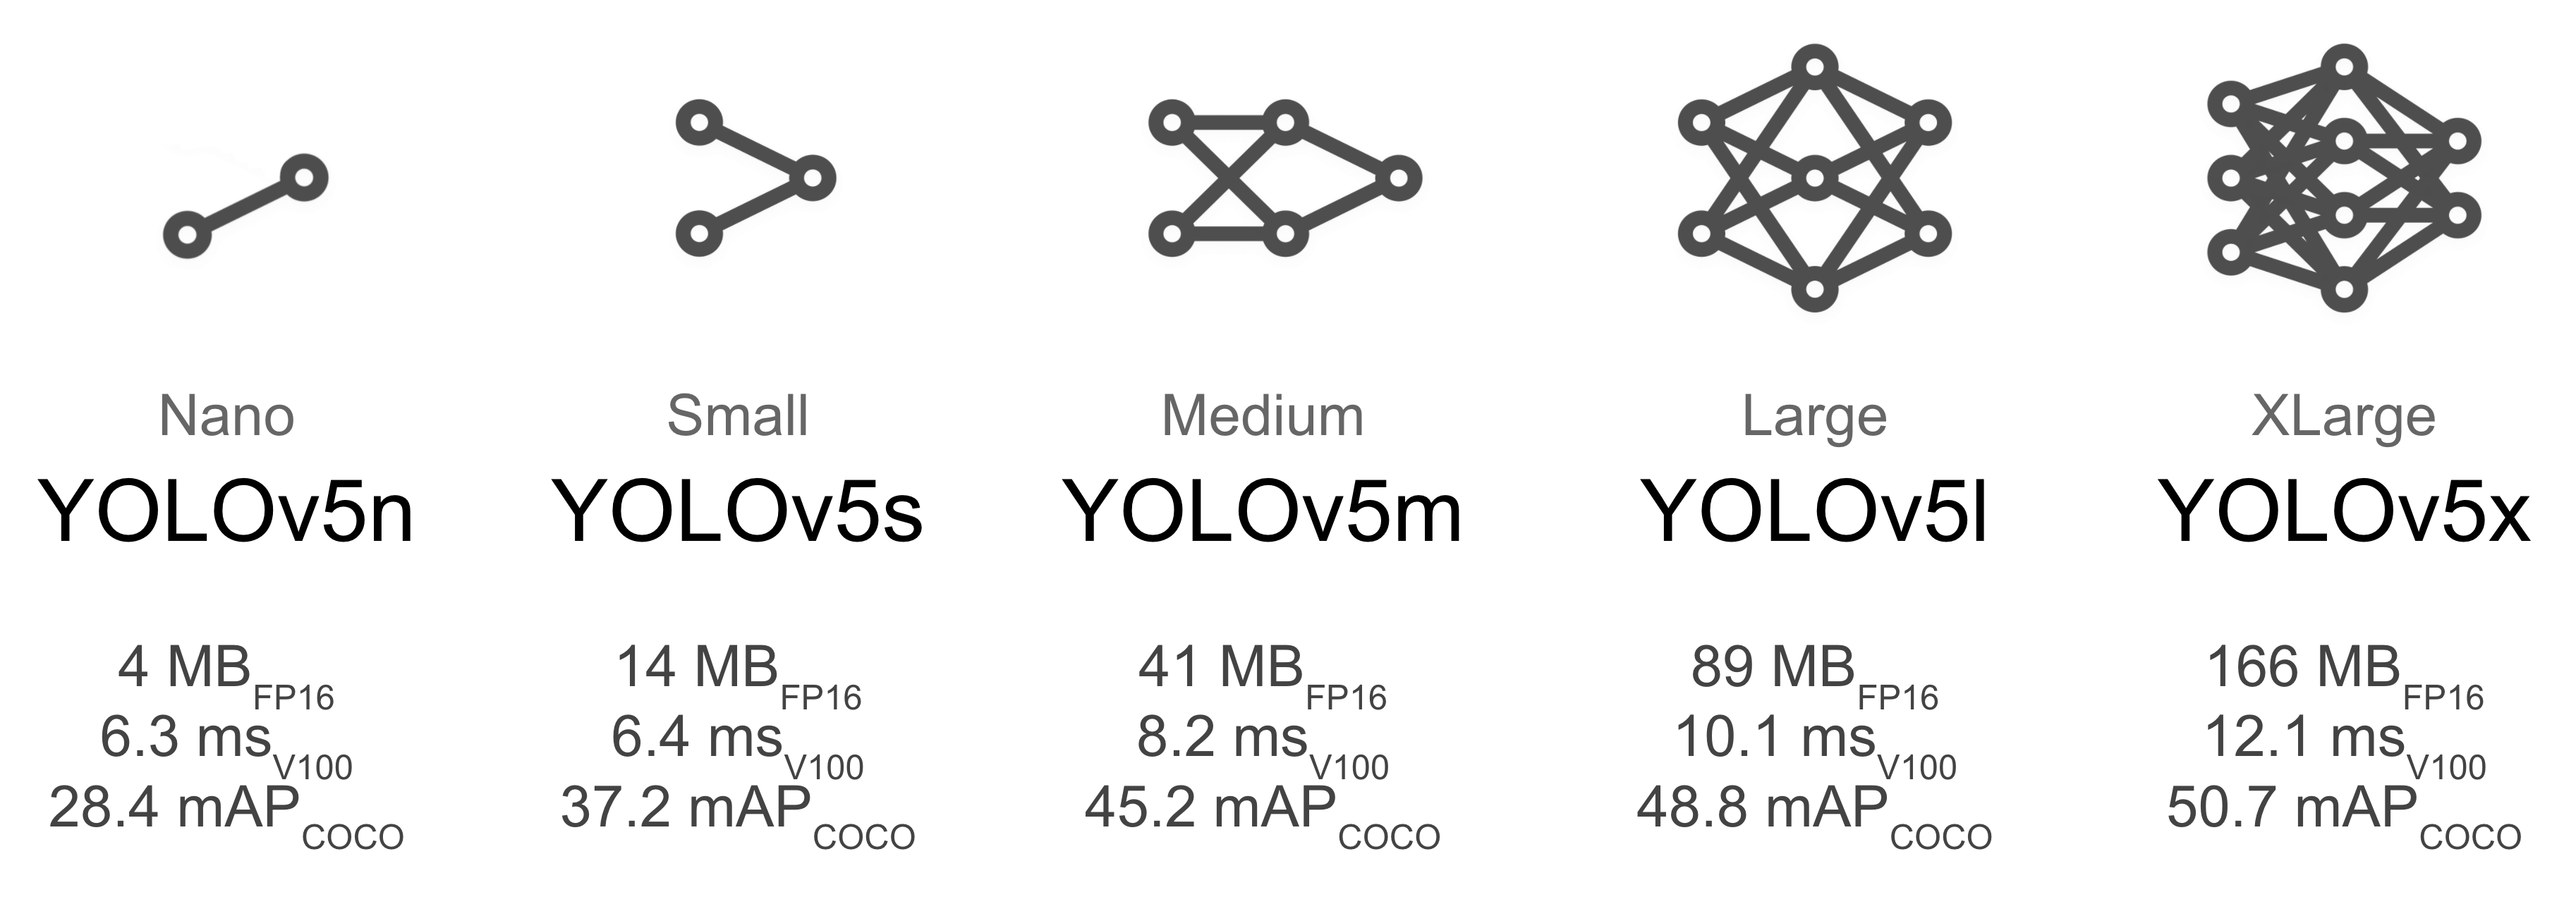
\includegraphics[width=0.9\linewidth]{figures/many_yolo.png} 
    \caption{Variants of YOLOv5.}
    \label{fig:many_yolo}
\end{figure}

YOLOv5 has several variants designed to balance accuracy, speed, and computational efficiency as shown in Figure~\ref{fig:many_yolo}, depending on the application:

\begin{itemize}
    \item \textbf{YOLOv5s (Small):} This is the smallest and fastest variant of YOLOv5. It is optimized for real-time performance on devices with limited computational resources. While it sacrifices some accuracy compared to larger models, it is highly suitable for use cases requiring high-speed processing, such as live video streaming or embedded systems.
    \item \textbf{YOLOv5m (Medium):} Trivial.
    \item \textbf{YOLOv5l (Large):} Trivial.
    \item \textbf{YOLOv5x (Extra Large):} The x-version is the largest model in the YOLOv5 series. It provides the highest detection accuracy, especially for small or densely packed objects. However, it also requires the most computational resources and may not be suitable for real-time processing on devices with limited hardware.
    \item \textbf{YOLOv5x6 (Extra Extra Large):} This is an even more powerful variant of YOLOv5x, designed for applications where accuracy is critical, and computational power is not a limiting factor. YOLOv5x6 is typically used for high-accuracy tasks like large-scale object detection in complex environments, though its speed is slower than smaller versions.
\end{itemize}

\subsection{Experiment result}

\begin{itemize}
    \item \textbf{YOLOv11:} 
    The latest advancement in state-of-the-art (SOTA) vision models. YOLOv11 combines speed, precision, and ease of use.
    \item \textbf{Road Sign Detection Dataset:}
    \begin{itemize}
        \item Contains 877 images of 4 distinct classes for the objective of road sign detection. \cite{make_ml}
    \end{itemize}
    \item \textbf{Data Process:}
    \begin{itemize}
        \item Auto-orient
        \item Resize to (640, 640)
        \item Noise augmentation
    \end{itemize}
    \item \textbf{Training Result:}
    \begin{itemize}
        \item \textbf{mAP:} 93.1\%
        \item \textbf{Precision:} 95.5\%
        \item \textbf{Recall:} 87.6\%
    \end{itemize}
\end{itemize}

\begin{figure*}[!t]
    \centering
    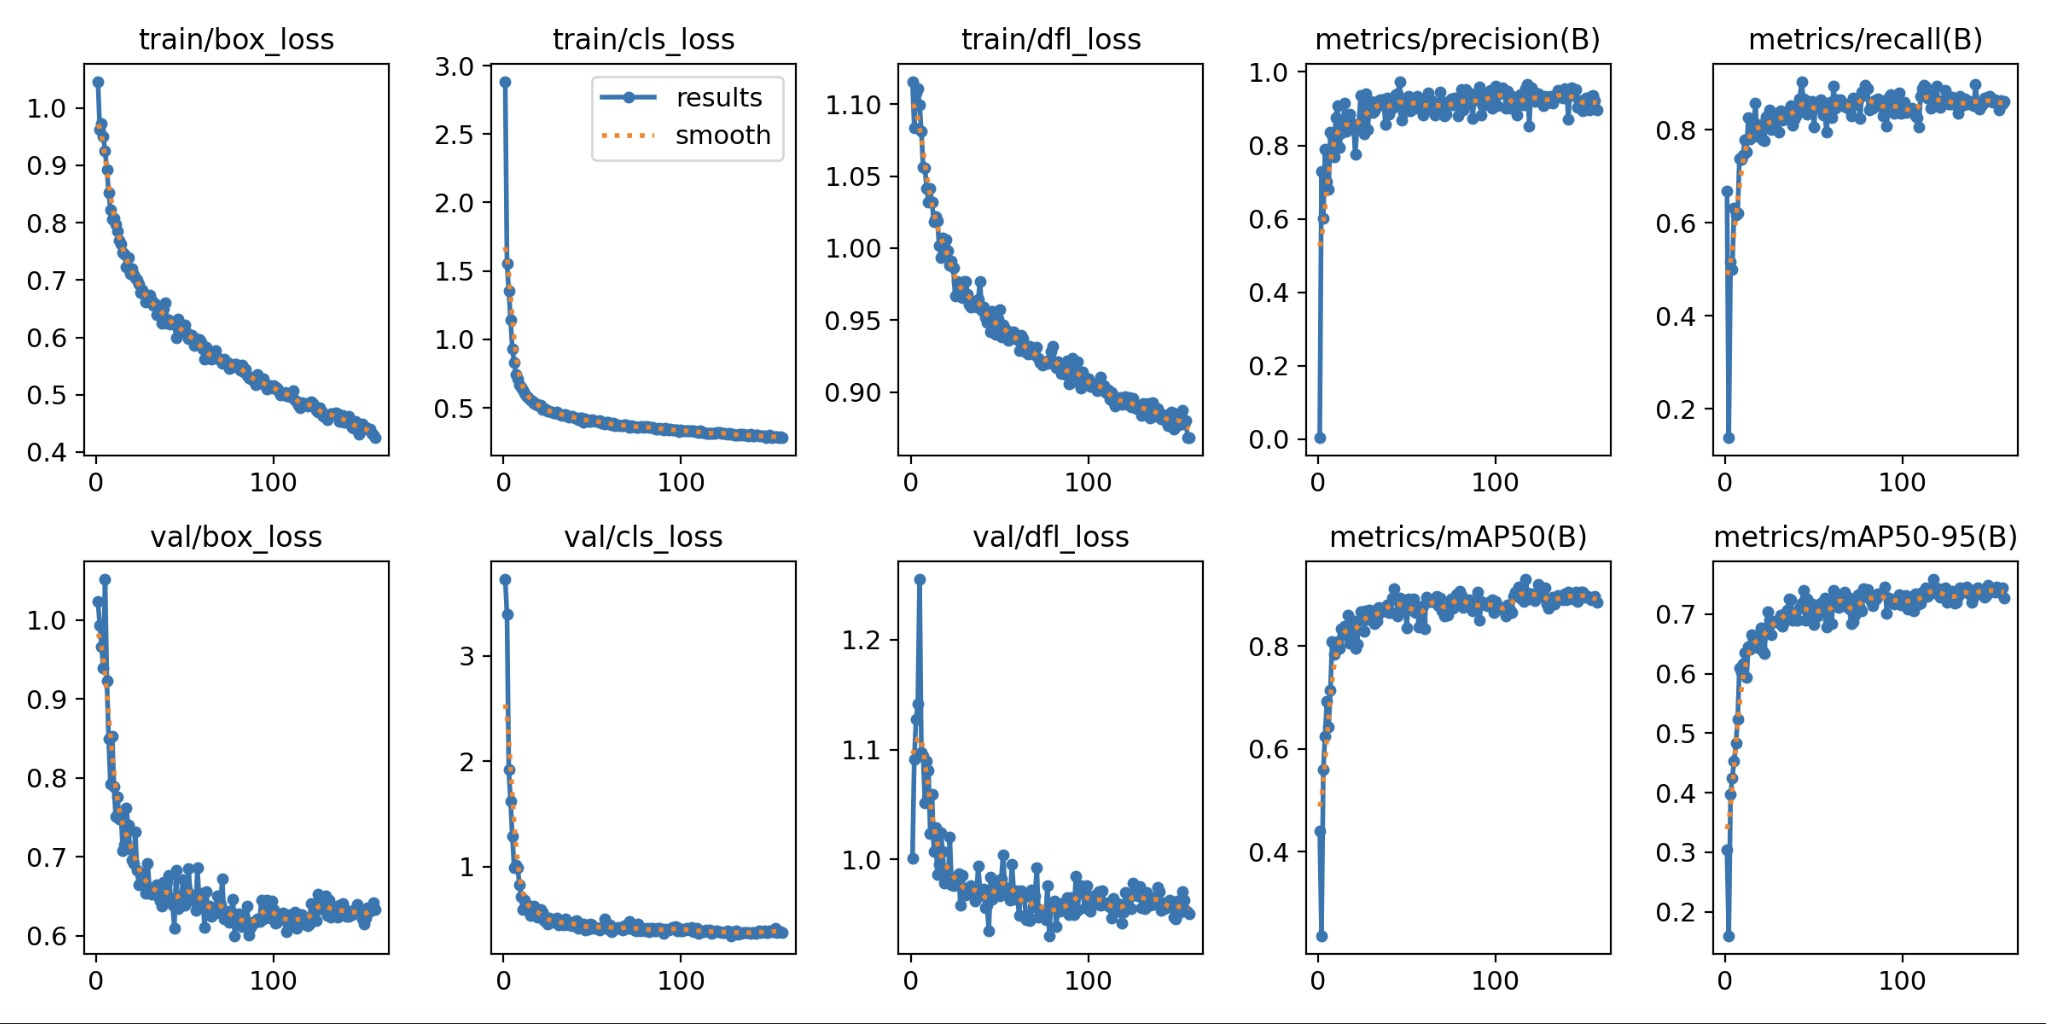
\includegraphics[width=0.9\linewidth]{figures/result.jpg} 
    \caption{Train Progress.}
    \label{fig:train_progress}
\end{figure*}

\begin{figure}[!t]
    \centering
    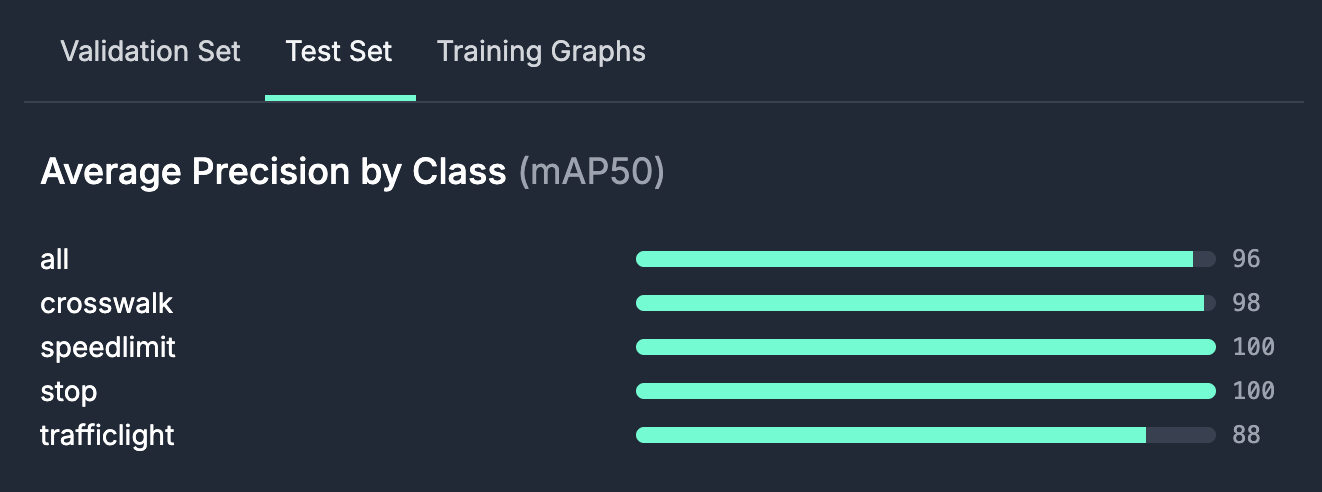
\includegraphics[width=0.9\linewidth]{figures/green1.png} 
    \caption{Validataion Metrix.}
    \label{fig:val_metrix}
\end{figure}

\begin{figure}[!t]
    \centering
    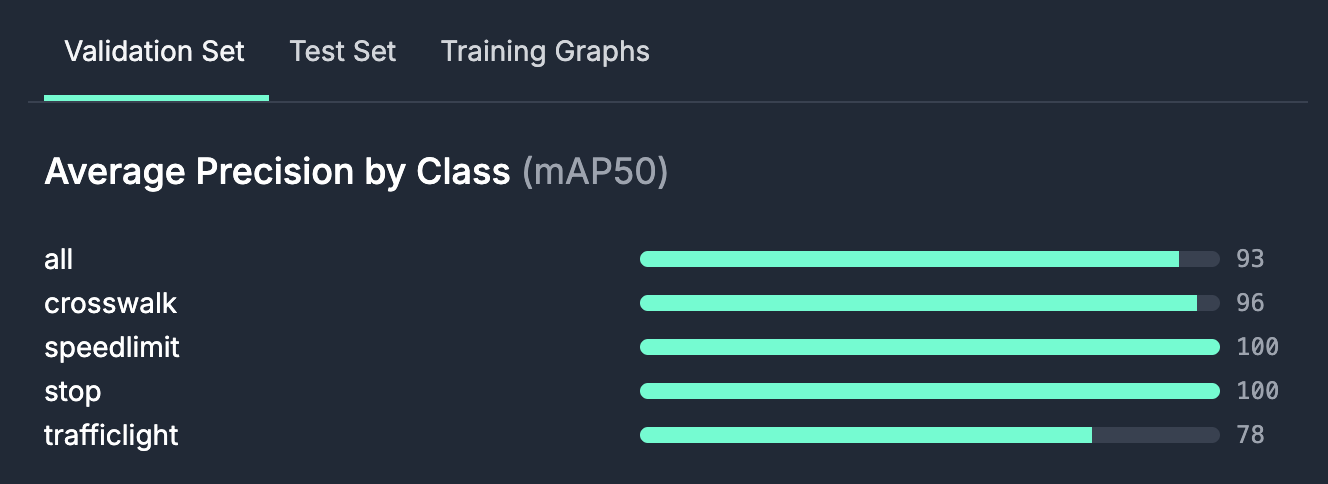
\includegraphics[width=0.9\linewidth]{figures/green2.png} 
    \caption{Train Metrix.}
    \label{fig:train_metrix}
\end{figure}

The results metrix of the YOLOv11 model on the Road Sign Detection Dataset are as follows (Figure~\ref{fig:train_progress}, Figure~\ref{fig:val_metrix}, Figure~\ref{fig:train_metrix}):

\
\section{Research Plan and Expected Results}
\hrulefill

\subsection{Time schedule}

The project timeline for Traffic Sign Detection and Recognition (TSDR) is outlined in Table~\ref{tab:timeline}:

\subsection{Expected results}

\begin{itemize}
    \item Use YOLO to perform regression and utilize Sill-net for light optimization and reclassification to achieve better accuracy compared with present results.
    \item Add attention modules (time, space, frequency, etc.) to YOLO to increase the accuracy of classification.
    \item The expected performance is to process real-world traffic sign images or video streams at 30 fps on a mobile phone device.
\end{itemize}

\begin{table}[H]
    \centering
    \caption{Project Timeline for Traffic Sign Detection and Recognition (TSDR)}
    \begin{tabular}{@{}llp{0.6\linewidth}@{}}
    \toprule
    \textbf{Date}         & \textbf{Week} & \textbf{Task Description}                                                                                                 \\ \midrule
    2024/10/24            & Week 7        & Project selection: TSDR problem (Traffic Sign Detection and Recognition).                                                 \\
    2024/11/11            & Week 8        & Midterm Preparation.                                                                                                      \\
    2024/11/7             & Week 9        & Reproduce provided reference paper individually. Read field background information and the latest paper overview. \\
                           &               & Collect dataset, test different methods and models.                                                                       \\
    2024/11/14            & Week 10       & Make comparison from previous work. Choose YOLOv5 as the base model of the project.                                       \\
    2024/11/21            & Week 11       & Train YOLOv5's branch models on the collected dataset. Analyze the training results.                                      \\
    2024/11/28            & Week 12       & Do Research Proposal and PPT. Summarize previous work and make plans for the following weeks.                             \\
    2024/12/5             & Week 13       & Clean the TT100K dataset and transform it to YOLO format, then train it on the YOLOv5 models.                             \\
                           &               & Compare experiment results with previous papers and work. Try to optimize and add plug-and-play modules to chosen model.  \\
                           &               & Analyze the differences and discuss further work.                                                                         \\
    2024/12/12            & Week 14       & Train the final optimized model and implement it on the device. Test it in real life and analyze the result.              \\
                           &               & Discuss further improvement in terms of real-life implementation.                                                        \\
    2024/12/19            & Week 15       & Write the final report and prepare for the presentation.                                                                  \\ \bottomrule
    \end{tabular}
    \end{table}

\
\section{Potential Challenges and Solutions}
\hrulefill

\subsection{Data Challenges}

\begin{figure*}[!t]
    \centering
    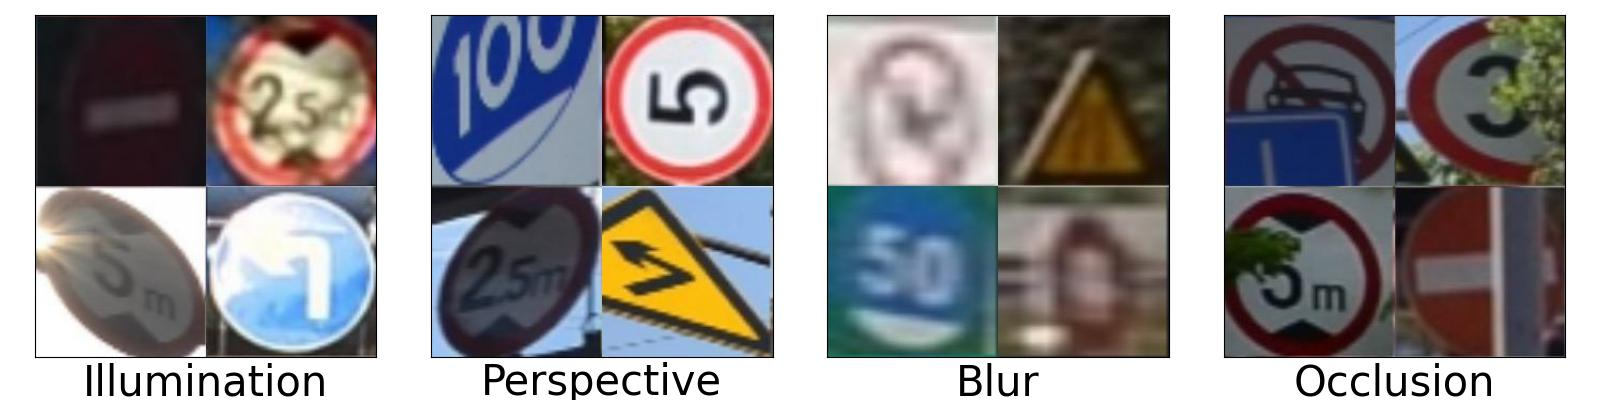
\includegraphics[width=0.9\textwidth]{figures/TT100K_bad_datas.jpg} 
    \caption{Examples of traffic sign data issue in TT100K.}
    \label{fig:data_issue}
\end{figure*}

As the examples shown in Figure~\ref{fig:data_issue} from TT100K dataset \cite{Zhe_2016_CVPR}, the data issues in traffic sign datasets are mainly caused by the following factors \cite{9072976}:

\subsubsection{Illumination Issues}\

Complex lighting variations caused by sunlight, vehicle headlights, streetlights, etc., can result in traffic signs being overexposed, underexposed, or obscured by shadows. Lighting variations affect the color, edges, and contrast of the target. Since recognizing color, edges, and contrast is critical for object detection algorithms, optimized preprocessing methods are necessary for addressing illumination issues in both traditional and neural network architectures.

For instance, analyzing the histogram distribution and statistical moments of the brightness channel can help understand the lighting conditions of an image. Contrast enhancement algorithms and illumination-invariant color models (e.g., HSV) can be used to sharpen edges and preserve color information under low-light conditions.

\subsubsection{Perspective Issues}\

The optical axis of installed cameras may not align perfectly with the target traffic signs, which can lead to image distortion. For example, a circular sign may appear elliptical, and edge lengths may look inconsistent.

The Generalized Hough Transform can largely handle distorted circles. Using an accumulator array and further filtering can resolve distorted or broken circles. For scale changes, scale-invariant features like SIFT and SURF can be employed. Oriented FAST and Rotated BRIEF (ORB) are widely used rotation- and scale-invariant features. Locally Encoded Shape Histograms (LESH) serve as a scale-invariant, shape-based object detection feature. Combining these methods with robust classifiers can address perspective distortions effectively.

\subsubsection{Motion Blur}\

Blurring issues can stem from low resolution, long distances, or camera motion, which weaken the clear edges in the image. Hence, restoration processes are required before detection.

Various algorithms have been developed to extract stable and clear edges from frames, such as optical flow and point spread function modeling. Frequency domain filtering using estimated motion models is also a method for motion blur restoration.

\subsubsection{Partial Occlusion}\

Traffic signs are often occluded by objects like lamp posts, billboards, trees, etc. However, their regular shapes and symmetry allow for detection even under partial occlusion.

Part-based object detection methods, local binary patterns, histograms of oriented gradients, and Randomized Hough Transform are effective algorithms for dealing with occluded signs (e.g., broken edges). Prediction-based tracking algorithms focus on edges rather than frames, resulting in lower error probabilities. Keypoint tracking and kernel-based tracking methods are commonly used for tracking occluded objects.

\subsection{Architecture Challenges}

The architecture-related challenges in traffic sign detection primarily arise due to model complexity, generalization issues, and integration requirements for real-world deployment. These challenges include the following:

\subsubsection{Dataset Limitations}\

The use of single datasets, such as GTSRB or TT100k, for training traffic sign detection models limits the model's ability to generalize to diverse environments. These datasets often fail to capture the diversity of real-world traffic signs, such as regional variations in shape, color, and condition. To enhance generalization, additional datasets with varied traffic sign types, environmental conditions, and geographic locations should be incorporated. Multi-domain learning or dataset augmentation techniques can also be employed to improve the model's robustness to unseen scenarios.

\subsubsection{Model Complexity}\

Integrating plug-and-play modules like Spatial Transformer Networks (STNs) into the model architecture increases its ability to handle geometric distortions and dynamic conditions. However, these modules also significantly increase computational overhead, requiring higher processing power and memory, which may hinder real-time deployment in resource-constrained environments such as embedded systems in autonomous vehicles. Optimizing the architecture to balance complexity and computational efficiency is critical for practical applications.

\subsubsection{Overfitting Risk}\

Overfitting occurs when a model becomes overly reliant on specific features of the training dataset, leading to poor performance on new or unseen data. Traffic sign datasets often lack sufficient diversity, exacerbating this issue. Techniques like data augmentation, dropout, weight regularization, and early stopping can mitigate overfitting. Additionally, transfer learning from large-scale pre-trained models can help generalize better to new data.

\subsubsection{Real-Time Performance}\

Deep learning models like YOLO offer high detection accuracy but often struggle with real-time deployment due to their computational resource requirements. For traffic sign detection, real-time inference is essential to ensure timely decision-making in autonomous vehicles. Model optimization techniques, such as pruning, quantization, and knowledge distillation, can help reduce computational demands while maintaining accuracy.

\subsubsection{Integration with Real-World Systems}\

Traffic sign detection systems must integrate seamlessly with other components of autonomous driving systems, such as path planning, obstacle detection, and decision-making modules. This integration requires the detection model to provide highly reliable results with low latency. Modular design and thorough testing across diverse driving conditions are essential for achieving robust system integration.

\subsubsection{Dynamic Environment Adaptability}\

Real-world driving environments are highly dynamic and change rapidly due to factors such as traffic flow, weather conditions, and road types (e.g., urban streets, highways, rural roads). Traffic sign detection models must adapt to these variations, ensuring consistent performance across scenarios like nighttime driving, rainy weather, or cluttered urban environments. Techniques such as multi-scale detection, adaptive feature extraction, and continual learning can enhance adaptability to dynamic environments.

\bibliographystyle{IEEEtran} 
\bibliography{references} 

\end{document}